{
Vi supplerer her, de grafer der er givet af ``The Web Gallery of Art''
(\url{http://www.wga.hu}), omhandlende deres samling
af kunstartikler. Graferne er hentet d. 04/01-2010, så de kan afgive
lidt fra den samling vi bruger i vores undersøgelse, da vi hentede alt
på deres hjemmeside medio oktober 2009. Graferne findes på
\url{http://www.wga.hu/database/statisti/index.html}.

\section{Grafer gældende for malerier i samlingen}
\begin{figure}[H]
    \setlength\fboxsep{0pt}
    \setlength\fboxrule{0.5pt}
    \centering
    \fbox{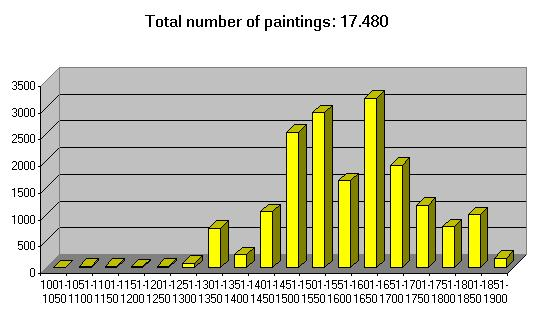
\includegraphics[width=0.8\textwidth]{bilag/billeder/wga.hu/paint_time-frame}}
    \caption[]{Painting Time-frame}
    \label{painting_timeframe}
\end{figure}

\begin{figure}[H]
    \setlength\fboxsep{0pt}
    \setlength\fboxrule{0.5pt}
    \centering
    \fbox{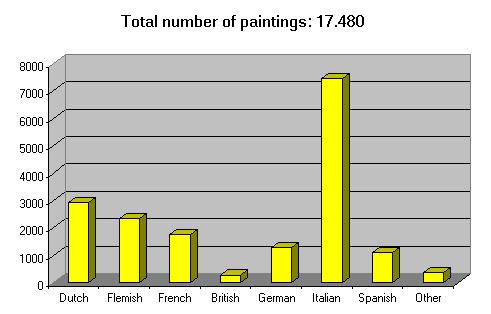
\includegraphics[width=0.8\textwidth]{bilag/billeder/wga.hu/paint_school}}
    \caption[]{Painting School}
    \label{painting_school}
\end{figure}

\begin{figure}[H]
    \setlength\fboxsep{0pt}
    \setlength\fboxrule{0.5pt}
    \centering
    \fbox{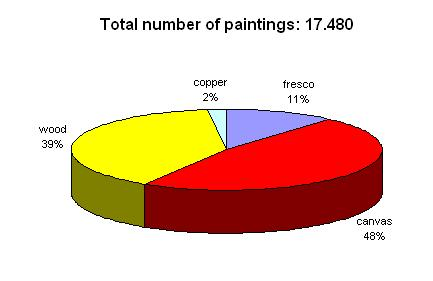
\includegraphics[width=0.8\textwidth]{bilag/billeder/wga.hu/paint_style}}
    \caption[]{Painting Technique}
    \label{painting_tech}
\end{figure}

\section{Grafer gældende hele samlingen}
\begin{figure}[H]
    \setlength\fboxsep{0pt}
    \setlength\fboxrule{0.5pt}
    \centering
    \fbox{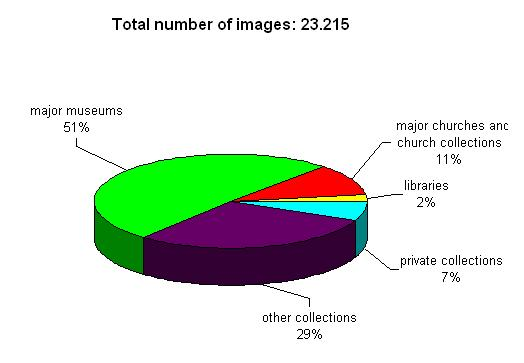
\includegraphics[width=0.8\textwidth]{bilag/billeder/wga.hu/collecti}}
    \caption[]{Collections}
    \label{collection_collection}
\end{figure}

\begin{figure}[H]
    \setlength\fboxsep{0pt}
    \setlength\fboxrule{0.5pt}
    \centering
    \fbox{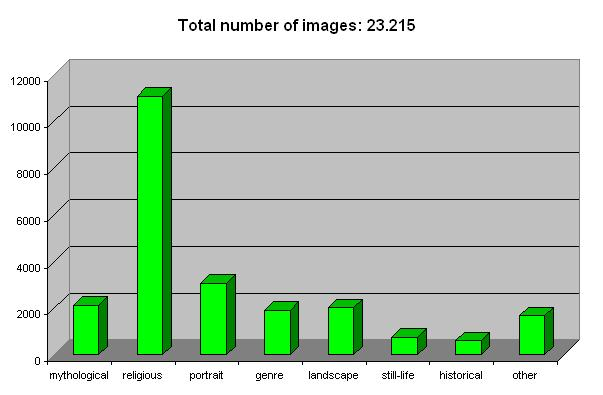
\includegraphics[width=0.8\textwidth]{bilag/billeder/wga.hu/subject}}
    \caption[]{Subject}
    \label{collection_subject}
\end{figure}

\begin{figure}[H]
    \setlength\fboxsep{0pt}
    \setlength\fboxrule{0.5pt}
    \centering
    \fbox{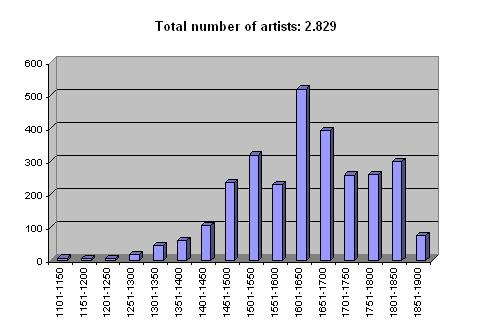
\includegraphics[width=0.8\textwidth]{bilag/billeder/wga.hu/artist_bd}}
    \caption[]{Artists active period}
    \label{Collection_born_died}
\end{figure}

}

% vim: set tw=72 spell spelllang=da:

